% Este formato está definido mais acima na seção "APARÊNCIA/FORMATAÇÃO"
% e só funciona com book/report, pois usa o nome dos capítulos nos cabeçalhos;
% se estiver usando article, comente ou troque por "plain"
\pagestyle{mainmatter}

% No texto principal, vamos usar espaçamento entre linhas padrão
\singlespacing
%\onehalfspacing

% Os capítulos de compõem a dissertação/tese, com numeração normal, podem
% ser inseridos diretamente aqui ou "puxados" de outros arquivos
%% ------------------------------------------------------------------------- %%n
\chapter{Introdução}
\label{cap:introducao}

\section{Contexto}
\label{sec:intro_contexto}

O estudo da planctologia é de grande importância na comunidade científica, principalmente na oceanografia. O nome plâncton vem do Grego planktos e significa errante, que vaga ou flutua. Caracteriza-se, assim, por organismos planctônicos os que não possuem o poder de locomoção suficiente para evitar o transporte passivo pelas massas de água [\cite{calazans2011organismos}].  A importância do estudo dessas criaturas se dá não somente por serem responsáveis por cerca de 45\% do oxigênio produzido mundialmente [\cite{brierleyplankton}],  através da fotossíntese do fitoplâncton, mas também pela grande diversidade de classes e de características como forma, tamanho e até da natureza do local de coleta [\cite{calazans2011organismos}]. 


Existem diversas maneiras de se fazer a amostragem de plânctons como, por exemplo, através de garrafas, redes, bombas de sucção e sistemas ópticos [\cite{calazans2011organismos}]. A amostragem de criaturas marítimas é datada desde de 1829, quando Thompson utilizou uma rede para coletar larvas de crustáceos e de cracas [\cite{brierleyplankton}]. Mas foi Victor Hensen, em 1887, o primeiro pesquisador a desenvolver, de fato, um sistema para coleta de amostragens de plânctons de forma quantitativa [\cite{benfield2007rapid, wiebe2003hensen, allen1919contribution}]. Naquela época estavam interessados em responder três questões fundamentais: Quais organismos planctônicos estão presentes no mar?  Quantos de cada tipo estão presentes? Como a composição dos plânctons muda com o passar do tempo?  [\cite{benfield2007rapid}]. Essas questões continuam atuais e graças ao avanço de sistemas e equipamentos de coleta, assim como de técnicas computacionais, há um grande esforço científico para a sua evolução. 


\section{Problema}
\label{sec:intro_problema}

Após a fase de coleta, especificamente através de sistemas ópticos, tem-se um conjunto de imagens de plânctons que não possuem rótulos. O grande desafio desse é que demanda-se muito tempo e pessoas especializadas para cumprir essa tarefa, já que elas possuem, por exemplo, uma grande variedade de classes, formas e tamanhos. Como resultado, normalmente temos uma lacuna muito grande entre o tempo de coleta das imagens e a rotulação que seja base para um classificador. Somado a isso, muitas vezes, já temos um novo equipamento que possuem fotos com características diferentes das anteriores. Ou seja, apesar de todo o avanço que tivemos com equipamentos e técnicas, esse ainda é um problema que ocorre desde 1800 [\cite{benfield2007rapid}]. Torna-se necessário, dessa forma, encontrar uma maneira de reduzir o esforço gasto em rotulação de amostras.  
    
O objetivo do aprendizado computacional é que tenhamos, no final do processo, um classificador que consiga determinar a qual classe alguma nova imagem um plâncton pertence. Isso só é possível quando temos uma base de treinamento. Para tanto é necessário que, dado as imagens coletadas, alguém as rotule. 


\section{Proposta}
\label{sec:intro_proposta}

Aprendizado Computacional é o estudo de sistemas que melhoram através da experiência. Dentro deste contexto existe, na literatura, algumas formas de trabalhar com nenhum ou pouco dados rotulados. Temos duas principais vertentes: Aprendizado Ativo e Aprendizado Semi-Supervisionado [\cite{zhu2006semi, abu2012learning}].  Este trabalho pretende mostrar que através de técnicas de aprendizado ativo conseguimos obter um bom classificador através 


\section{Trabalhos Relacionados}
\label{sec:intro_relacionados}

Texto texto texto texto texto texto texto texto texto texto texto texto texto texto texto texto texto texto texto texto texto texto texto texto texto texto


\section{Organização}
\label{sec:intro_organizacao}

Texto texto texto texto texto texto texto texto texto texto texto texto texto texto texto texto texto texto texto texto texto texto texto texto texto texto
\par

\chapter{Usando o \LaTeX{} e este modelo}

Não é necessário que o texto seja redigido usando \LaTeX{}, mas é fortemente
recomendado o uso dessa ferramenta, pois ela facilita diversas etapas do
trabalho e o resultado final é muito bom\footnote{O uso de um sistema de
controle de versões, como mercurial (\url{mercurial-scm.org}) ou git
(\url{git-scm.com}), também é altamente recomendado.}. Este modelo inclui
vários comentários explicativos e pacotes interessantes para auxiliá-lo com
ele.

O modelo é composto por estes arquivos:

\begin{itemize}
  \item Arquivo principal:
  \begin{itemize}
    \item \texttt{tese-exemplo.tex} (leia os comentários neste arquivo!)
  \end{itemize}

  \item Arquivo com as \textit{packages} usadas e suas configurações:
  \begin{itemize}
    \item \texttt{miolo-preambulo.tex} (leia os comentários neste arquivo!)
  \end{itemize}

  \item Arquivos com formato sugerido de capa, resumo e outros elementos:
  \begin{itemize}
    \item \texttt{imeusp.sty} (configurações de formatação -- não é preciso editar)
    \item \texttt{metadados-tese.tex} (é preciso inserir os metadados aqui)
    \item \texttt{folhas-de-rosto.tex} (resumo, dedicatória etc.)
  \end{itemize}

  \item Arquivos dos capítulos e apêndice:
  \begin{itemize}
    \item \texttt{cap-introducao.tex}
    \item \texttt{cap-latex.tex}
    \item \texttt{cap-tutorial.tex}
    \item \texttt{cap-exemplos.tex}
    \item \texttt{cap-conclusoes.tex}
    \item \texttt{ape-conjuntos.tex}
  \end{itemize}

  \item Diretório de figuras:
  \begin{itemize}
    \item \texttt{./figuras/}
  \end{itemize}

  \item Outros arquivos auxiliares:
  \begin{itemize}
    \item \texttt{bibliografia.bib} (arquivo de dados bibliográficos)
    \item \texttt{plainnat-ime.bbx} (estilo plainnat para bibliografias com biblatex)\index{biblatex}
    \item \texttt{plainnat-ime.cbx} (estilo plainnat para citações com biblatex)
    \item \texttt{plainnat-ime.bst} (estilo plainnat para bibliografias com bibtex)\index{bibtex}
    \item \texttt{alpha-ime.bst} (estilo alpha para bibliografias com bibtex)\index{bibtex}
    \item \texttt{natbib-ime.sty} (tradução da \textit{package} padrão natbib -- citações com bibtex)\index{natbib}
    \item \texttt{hyperxindy.xdy} (arquivo de configuração para hiperlinks no índice remissivo)
    \item \texttt{Makefile} (arquivo que automatiza a geração do documento com o comando \textsf{make})
    \item \texttt{latexmkrc} (arquivo que automatiza a geração do documento com o comando \textsf{latexmk})
  \end{itemize}
\end{itemize}

Para compilar o documento, basta executar o comando \textsf{latexmk} (ou
\textsf{make}). Talvez seu editor ofereça uma opção de menu para compilar o
documento, mas ele provavelmente depende do \textsf{latexmk} para isso.
\LaTeX{} gera diversos arquivos auxiliares durante a compilação que, em
algumas raras situações, podem ficar inconsistentes (causando erros de
compilação ou erros no PDF gerado, como referências faltando ou numeração de
páginas incorreta no sumário). Nesse caso, é só usar o comando
\textsf{latexmk -C} (ou \textsf{make clean}), que apaga todos os arquivos
auxiliares gerados, e em seguida rodar \textsf{latexmk} (ou \textsf{make})
novamente.

\section{Instalação do \LaTeX{}}

\LaTeX{} é, na verdade, um conjunto de programas. Ao invés de procurar e
baixar cada um deles, o mais comum é baixar um pacote com todos eles juntos.
Há dois pacotes desse tipo disponíveis: MiK\TeX{} (\url{miktex.org}) e
\TeX{}Live (\url{www.tug.org/texlive}). Ambos funcionam em Linux, Windows e
MacOS X. Em Linux, \TeX{}Live costuma estar disponível para instalação junto
com os demais opcionais do sistema. Em MacOS X, o mais popular é o Mac\TeX{}
(\url{www.tug.org/mactex/}), a versão do \TeX{}Live para MacOS X.  Em Windows,
o mais comumente usado é o MiK\TeX{}.

Por padrão, eles não instalam tudo que está disponível, mas sim apenas os
componentes mais usados, e oferecem um gestor de pacotes que permite adicionar
outros. Embora uma instalação completa do \LaTeX{} seja relativamente grande
(perto de 5GB), em geral vale a pena instalar a maior parte dos pacotes. Se
você preferir uma instalação mais ``enxuta'', não deixe de incluir todos os
pacotes necessários para este modelo. Por exemplo, no debian:

\begin{description}
  \item [inconsolata] -- está incluído em ``texlive-fonts-extra''
  \item [siunitx] -- está incluído em ``texlive-science''
  \item [biblatex] -- está incluído em ``texlive-bibtex-extra''
  \item [biber] -- é um pacote separado
  \item [xindy] -- é um pacote separado
\end{description}

Também é muito importante ter o \textsf{latexmk} (ou o \textsf{make}). No Linux,
a instalação é similar à de outros programas. No MacOS X e no Windows,
\textsf{latexmk} pode ser instalado pelo gestor de pacotes do MiK\TeX{} ou
\TeX{}Live. Observe que ele depende da linguagem \textsf{perl}, que precisa ser
instalada à parte no Windows (\url{www.perl.org/get.html}).

\section{Bibliografia}

Você pode usar referências bibliográficas nos formatos ``alpha'' ou ``plainnat''.
Se estiver usando natbib+bibtex\index{natbib}\index{bibtex}, use os arquivos .bst
``alpha-ime.bst'' ou ``plainnat-ime.bst'', que são versões desses dois formatos
traduzidas para o português. Se estiver usando biblatex\index{biblatex}
(recomendado), escolha o estilo ``alphabetic'' (que é um dos estilos padrão do
biblatex) ou ``plainnat-ime''. O arquivo de exemplo inclui todas essas opções;
basta des-comentar as linhas correspondentes e, se necessário, modificar o
arquivo Makefile para chamar o bibtex\index{bibtex} ao invés do
biber\index{biber} (este último é usado em conjunto com o biblatex).

\section{Perguntas Frequentes sobre o Modelo}

\begin{itemize}

\item \textbf{Posso usar pacotes \LaTeX{} adicionais aos sugeridos, como por exemplo: pstricks, pst-all, etc?}\\
Com certeza! Você pode modificar o arquivo o quanto desejar. O modelo \LaTeX{} serve só como uma ajuda inicial para o seu trabalho.

\item \textbf{As figuras podem ser colocadas no meio do texto ou devem ficar no final dos capítulos?}\\
Em geral as figuras devem ser apresentadas assim que forem referenciadas. Colocá-las no final dos capítulos dificultaria um pouco a leitura, mas isso depende do estilo do autor, orientador, ou lugar de publicação. Converse com seu orientador!

\item \textbf{Existe algo específico para citações de páginas web?}\\
Biblatex define o tipo ``online''; bibtex\index{bibtex}, por padrão, não tem um tipo específico. Se o que você está citando não é um texto específico mas sim um sítio, como por exemplo o sítio de uma empresa ou de um produto, pode ser mais adequado colocar a referência como nota de rodapé e não na lista de referências; nesses casos, algumas pessoas acrescentam uma segunda lista de referências especificamente para recursos \emph{online} (biblatex \index{biblatex} permite criar múltiplas bibliografias). Se, no entanto, trata-se de um texto específico, como uma postagem em um blog, uma matéria jornalística ou mesmo uma mensagem de email para uma lista de discussão, a citação deve seguir o formato de outros tipos de documento e informar título, autor etc. Normalmente usa-se o campo ``howpublished'' para especificar que se trata de um recurso \emph{online}. Observe também que artigos que fazem parte de uma publicação, como os anais de um congresso, e que estão disponíveis \emph{online} devem ser citados por seu tipo verdadeiro e apenas incluir o campo ``url'' (não é nem necessário usar o comando \textsf{\textbackslash{}url\{\}}), aceito por todos os tipos de documento do bibtex/biblatex.

\item \textbf{A bibliografia está sendo impressa em inglês (usa ``and'' ao invés de ``e'' para separar os nomes dos autores)}\\
Você deve estar usando um estilo de bibliografia bibtex diferente dos sugeridos. Uma simples solução é copiar o arquivo de estilo correspondente da sua instalação \LaTeX{} para o diretório onde seus arquivos estão e mudar ``and'' por ``e'' (ou ``\&'' se preferir) na função format.names. Biblatex tem pleno suporte a diferentes línguas e é possível personalizar as traduções (há um exemplo no modelo).

\item \textbf{Aparece uma folha em branco entre os capítulos}\\
Essa característica foi colocada propositalmente, dado que todo capítulo deve (ou deveria) começar em uma página de numeração ímpar (lado direito do documento). Acrescente ``openany'' como opção da classe, i.e., \textsf{\textbackslash{}documentclass[openany,11pt,twoside,a4paper]\{book\}}.

\item \textbf{É possível resumir o nome das seções/capítulos que aparece no topo das páginas?}\\
Sim, usando a sintaxe \textsf{\textbackslash{}section[mini-titulo]\{titulo enorme\}}. Isso é especialmente útil nos \textit{captions}\index{Legendas} das figuras e tabelas, que muitas vezes são demasiadamente longos para a lista de figuras/tabelas.

\item \textbf{Existe algum programa para gerenciar referências em formato bibtex?}\\
Sim, há vários. Uma opção bem comum é o JabRef; outra é usar Zotero\index{Zotero} ou Mendeley\index{Mendeley} e exportar os dados deles no formato .bib.

\item \textbf{Como faço para usar o Makefile (comando make) no Windows?}\\
Se você instalou o \LaTeX{} usando o Cygwin, você já deve ter o comando make instalado; se não, tente o MSYS2. Se você pretende usar algum dos editores sugeridos, é possível deixar a compilação a cargo deles, dispensando o uso do make.
\end{itemize}

\par

% Vamos definir alguns comandos auxiliares para facilitar.

% "textbackslash" é muito comprido.
\newcommand{\sla}{\textbackslash}

% Vamos escrever comandos (como "make" ou "itemize") com formatação especial.
\newcommand{\cmd}[1]{\textsf{#1}}

% Idem para packages; aqui estamos usando a mesma formatação de \cmd,
% mas poderíamos escolher outra.
\newcommand{\pkg}[1]{\textsf{#1}}

% A maioria dos comandos LaTeX começa com "\"; vamos criar um
% comando que já coloca essa barra e formata com "\cmd".
\newcommand{\ltxcmd}[1]{\cmd{\sla{}#1}}

\chapter{Do zero ao mínimo com \LaTeX{}}

Preparar um texto para impressão envolve duas coisas:

\begin{description}
\item[Escrever:] digitar, recortar/colar trechos, revisar etc.
\item[Formatar:] definir o tamanho da fonte, o
espaçamento entre parágrafos etc.
\end{description}

Hoje é comum fazer essas duas coisas ao mesmo tempo, graças à visualização
imediata que o computador oferece. No entanto, imagine como era o processo de
produção de um livro nos anos 1970: o autor escrevia seu texto em uma máquina
de escrever e enviava esse material para o editor, que era responsável pela
tarefa de formatá-lo para impressão. O autor muitas vezes inseria anotações
para o editor explicando coisas como ``este parágrafo é uma citação'', e o
editor criava algum mecanismo visual para representar isso.

Não é de se surpreender que, com o surgimento do microcomputador, os primeiros
programas para criação de textos seguissem um funcionamento similar: o autor
digitava e editava seu texto sem formatá-lo visualmente, apenas inserindo
alguns comandos correspondentes a aspectos da formatação que ele depois
revisava na versão impressa. \LaTeX{} é uma ferramenta baseada nesse processo:
você prepara seu texto no editor de sua preferência, insere comandos no texto
que indicam a estrutura do documento e o processa com o \LaTeX{}, que gera um
arquivo PDF formatado. Embora seja um estilo ``antigo'' de trabalhar, ele é
muito eficiente em vários casos. Ou seja, dependendo da situação, pode ser
mais adequado trabalhar fazendo tudo ao mesmo tempo ou dividindo o trabalho
nessas duas fases. De maneira geral:

\begin{itemize}
\item Se você precisa criar páginas diferentes entre si com \emph{layout}
definido manualmente, é melhor usar uma ferramenta que permita trabalhar
visualmente, como LibreOffice Writer, MS-Word, Google Docs etc.;

\item Se você precisa fazer um documento relativamente longo com estrutura
regular (capítulos, seções etc.), é melhor usar ferramentas que formalizam
essa estrutura (como \LaTeX{}) ao invés de usar ferramentas visuais;

\item Se você precisa fazer um documento envolvendo referências cruzadas,
bibliografia relativamente extensa ou fórmulas matemáticas, é difícil
encontrar outra ferramenta tão eficiente quanto \LaTeX{};

\item Se você precisa criar um documento simples, ambas as abordagens
funcionam bem; cada um escolhe esta ou aquela em função da familiaridade
com as ferramentas;

\item Se você quer que a qualidade tipográfica do resultado seja realmente
excelente, é necessário usar uma ferramenta profissional, como \LaTeX{},
Scribus, Adobe InDesign ou outras; processadores de texto convencionais não
oferecem o mesmo nível de qualidade dessas ferramentas.
\end{itemize}

\section{Visão Geral}

Com \LaTeX{}, você prepara o texto (incluindo as indicações de estrutura) em
um editor de textos qualquer, salva como arquivo de texto puro (``.txt'',
mas é comum usar a extensão ``.tex'' ao invés de ``.txt'') e processa esse
arquivo com o comando ``pdflatex'' (``compila'' o documento) para obter o
PDF correspondente. Qualquer editor capaz de salvar arquivos em formato
texto puro, como o bloco de notas do windows, vim, emacs etc. pode ser usado.
Programas como LibreOffice Writer, MS-Word etc. também funcionam, mas
possivelmente vão gerar dores de cabeça porque vão tentar formatar algumas
coisas automaticamente (e de maneira incompatível com \LaTeX{}).

Se você preferir, existem editores projetados especificamente para trabalhar
com \LaTeX{}; eles em geral utilizam cores para distinguir o texto dos
comandos de formatação, automatizam o processo de compilação do documento e
oferecem outras comodidades. Os mais comumente usados são \TeX{}maker,
\TeX{}studio e \TeX{}works; os três são software livre e funcionam em
Windows, MacOS e Linux. \TeX{}nicCenter é outra opção livre, mas funciona
apenas em Windows. O editor atom (\url{atom.io}) tem uma interface às vezes
peculiar para não programadores, mas em conjunto com as suas \emph{packages}
\pkg{atom-latex}, \pkg{latex-document-outline},
\pkg{grammar-token-limit} e \pkg{preview-inline}, ele é uma boa opção
(observe que essas são \emph{packages} do atom, não do \LaTeX{}). O mesmo
vale para o editor emacs (\url{www.gnu.org/software/emacs}) e sua package
\pkg{AUC\TeX{}}. Ainda outra possibilidade são os editores \emph{online},
como overleaf (\url{www.overleaf.com}) e sharelatex (\url{www.sharelatex.com}).

\LaTeX{} ignora quebras de linha e trata sequências de vários espaços como
se fossem apenas um. Isso significa que você pode usar quebras de linha e
espaços no texto que está digitando como ``dicas visuais'' da estrutura do
texto durante a edição. É muito comum fazer isso com listas de itens, por
exemplo. Uma ou mais linhas em branco sinalizam o fim de um parágrafo e o
início de outro. O caractere ``\%'' indica que o restante da linha é um
comentário, ou seja, um trecho de texto que não tem nenhum efeito sobre o
resultado final do documento. Comentários podem ser usados como lembrete sobre
alguma decisão, para indicar um parágrafo que ainda precisa de revisão etc.
Por conta desse significado especial, para inserir um caractere \% ``normal''
no texto é preciso digitar ``\ltxcmd{\%}''.

Um documento \LaTeX{} é dividido em duas partes: o \emph{preâmbulo}, onde
você coloca comandos de configuração para o documento, e o \emph{corpo} do
documento em si, que contém o texto propriamente dito. O preâmbulo é onde
você define as características do resultado tipográfico esperado: tipo e
tamanho da fonte a usar, posição dos títulos e subtítulos na página etc.
Como definir todas as configurações de impressão desejadas é bastante complexo,
\LaTeX{} fornece algumas pré-definições padrão (``\emph{classes}'') em
função do tipo de documento, que você escolhe com o comando
\ltxcmd{documentclass\{nome-da-classe\}} no preâmbulo. As principais classes
são \pkg{book}, \pkg{report} e \pkg{article}; você pode saber mais sobre elas
(e outras) em qualquer texto introdutório sobre \LaTeX{} na Internet.
\pkg{book} e \pkg{report} são as mais adequadas para a escrita de teses ou
dissertações acadêmicas.

\LaTeX{} também tem \emph{packages} (``\emph{plugins}'') que acrescentam
funcionalidades ou modificam as classes padrão e também são carregadas no
preâmbulo, com o comando \ltxcmd{usepackage\{nome-da-package\}}. Várias
delas podem receber opções adicionais no formato
\ltxcmd{usepackage[opção1,opção2...]\{nome-da-package\}}; a documentação
de cada package detalha as opções disponíveis.

Qualquer documento \LaTeX{} utiliza várias packages, portanto é preciso
conhecê-las. Isso às vezes é trabalhoso porque algumas delas podem se
tornar obsoletas e, com isso, sítios web com ``dicas'' podem estar
desatualizados. O sítio \url{www.ctan.org} é um índice com praticamente
todas as packages disponíveis, incluindo sua documentação. Além dessas,
é comum que revistas científicas ofereçam packages que pré-definem a
formatação esperada para os artigos. Finalmente, o sítio
\url{tex.stackexchange.com} é um fórum de perguntas e respostas sobre
\LaTeX{} que é muito útil.

Usar algum documento existente como base para criar seu texto em geral é
uma boa ideia; o IME/USP oferece um modelo adequado para teses e
dissertações (\url{github.com/LSS-USP/modelo-latex}) que pode ser
adaptado para outros usos e outras instituições. Há também um modelo
(\url{www.abntex.net.br}) que procura seguir as normas da ABNT para
documentos científicos.

\section{Comandos Básicos}
\label{sec:basico}

Como mencionado anteriormente, \LaTeX{} divide o trabalho de produção
de um texto entre a preparação do conteúdo e a definição da forma de
apresentação. Assim, os comandos usados durante a produção do conteúdo
procuram expressar o \emph{significado} de cada elemento, e não sua
aparência. Por exemplo, para realçar uma palavra é comum usar texto
\textit{em itálico}; embora exista um comando especificamente para gerar
textos em itálico em \LaTeX{}, o recomendado é que se utilize o comando
\ltxcmd{emph} (``enfatizado''), pois em alguns casos pode ser melhor
utilizar \textbf{negrito}, \textsc{Small Caps} ou outro mecanismo para
dar ênfase a uma palavra. Essa é uma orientação geral para a escrita de
textos com \LaTeX{}: procure definir a estrutura, não a aparência.

Um exemplo de documento \LaTeX{} simples:

\begin{verbatim}
        % O documento começa com o preâmbulo
        % Vamos usar a classe "book" com fonte no tamanho 11pt
        \documentclass[11pt]{book}
        % Vamos usar caracteres acentuados
        \usepackage[utf8]{inputenc}
        % Vamos escrever em português do Brasil
        \usepackage[brazil]{babel}
        % Estas linhas não imprimem nada, apenas definem
        % os valores que serão usados por "\maketitle"
        \author{Fulano de Tal}
        \title{Começando a usar o \LaTeX{}}
        % Finaliza o preâmbulo e inicia o conteúdo:
        \begin{document}
        % Cria uma página de título com os dados definidos acima
        \maketitle
        % Capítulos, seções etc. são numerados automaticamente
        \chapter{Cheguei!}
        Oi, Galera!
        % É preciso sinalizar o final do documento
        \end{document}
\end{verbatim}

Esse exemplo mostra como definir o nome de um capítulo. Existem também os
comandos \ltxcmd{section}, \ltxcmd{subsection}, \ltxcmd{subsubsection} e
\ltxcmd{paragraph} (a classe \pkg{book} inclui também \ltxcmd{part}, um nível
acima de \ltxcmd{chapter}). Usar o nome do comando seguido de um asterisco
(\ltxcmd{chapter*} etc.) faz o capítulo/seção não ser numerado nem incluído
no sumário (nem considerado na contagem de capítulos, seções etc.).

Para criar listas de itens, você pode fazer\footnote{Observe o uso de
espaços no início das linhas com \ltxcmd{item} para deixar a
estrutura visualmente mais clara durante a edição.}:

\begin{verbatim}
        \begin{itemize}
            \item Primeiro item
            \item Segundo item
            \item Terceiro item
        \end{itemize}
\end{verbatim}

Além de ``itemize'', há também ``enumerate'' (auto-explicativo) e ``description'':

\begin{verbatim}
        \begin{description}
            \item[O primeiro item] é o primeiro;
            \item[O segundo item] é o segundo;
            \item[O terceiro item] é o terceiro.
        \end{description}
\end{verbatim}

Citações curtas normalmente são incluídas no fluxo normal do texto e colocadas
entre aspas; para citações mais longas, use \ltxcmd{begin\{quote\}} ou
\ltxcmd{begin\{quotation\}} (este último é mais adequado para citações com
vários parágrafos). Para poesia, use \cmd{verse} (estrofes são separadas por
uma linha em branco e versos são separados por \cmd{\sla\sla{}*}. O asterisco
é opcional; ele instrui \LaTeX{} a manter as linhas na mesma página). A package
\pkg{csquotes} acrescenta recursos sofisticados para citações.

Para inserir uma nota de rodapé, use o comando
\ltxcmd{footnote\{texto da nota\}}\index{Notas de rodapé}. Um espaço
não-separável é indicado pelo caractere til (``\cmd{\textasciitilde{}}'')
e é possível forçar uma quebra de linha com ``\cmd{\sla\sla{}}''. Aspas
tipográficas (``'' e `') são inseridas com
% As fontes Linux Libertine e inconsolata não têm estes caracteres
\texttt{\textasciigrave\textasciigrave\textquotesingle\textquotesingle} e
\texttt{\textasciigrave\textquotesingle}. Você pode consultar a lista completa de
símbolos em \url{www.ctan.org/tex-archive/info/symbols/comprehensive/symbols-a4.pdf}.
Uma outra maneira de encontrar símbolos é usar este sítio: \url{detexify.kirelabs.org/classify.html}.

\section{Referências Cruzadas e \emph{Floats}}
\label{sec:refs}

É comum que um trecho do texto faça referência a outro trecho (``como
discutimos no capítulo~X\ldots''). Isso pode ser feito diretamente, mas
se você reorganizar o documento ou acrescentar seções, a numeração pode
mudar. Para evitar esse problema, você pode gerar essas referências
automaticamente com o par de comandos \ltxcmd{label\{nome-sugestivo\}} e
\ltxcmd{ref\{nome-sugestivo\}} (para o número da seção/capítulo) ou
\ltxcmd{pageref\{nome-sugestivo\}} (para o número da página).

Esse mecanismo também é muito útil para figuras e tabelas.
É claro que o ideal seria que tabelas e figuras sempre aparecessem junto ao
texto a que se referem. No entanto, isso é impossível por conta da divisão
do texto em páginas. Em \LaTeX{}, figuras e tabelas são incluídas como
\emph{floats} (localização flexível) usando \ltxcmd{begin\{figure\}}
e \ltxcmd{begin\{table\}} e o programa procura o ``melhor''
lugar para colocá-las. Dentro do \emph{float} é inserido um
\ltxcmd{label} para que se possa fazer referência à figura/tabela
no texto (com o comando \ltxcmd{ref}). A figura/tabela em
si é definida com \ltxcmd{includegraphics} ou \ltxcmd{begin\{tabular\}},
e em geral é uma boa ideia acrescentar uma descrição com
\ltxcmd{caption}\index{Legendas}.

\LaTeX{}\index{Floats!Ordem} garante que a sequência das figuras e a
sequência das tabelas sejam respeitadas (a Figura~6 nunca aparece depois da
Figura~7). No entanto, isso \emph{não} se aplica a \emph{floats} de tipos
diferentes, ou seja, se você definiu a Figura~5, a Tabela~3 e a Figura~6,
elas podem aparecer no documento na ordem ``Figura~5, Tabela~3, Figura~6'',
``Figura~5, Figura~6, Tabela~3'' ou ``Tabela~3, Figura~5, Figura~6''.

\section{Múltiplas Execuções e Comandos Auxiliares}

\LaTeX{} numera capítulos, seções, figuras etc. automaticamente
e pode fazer referências a seções ou figuras que aparecem tanto antes
quanto depois da própria referência. Para isso funcionar, o trabalho de
geração do arquivo final é dividido em duas partes: primeiro, a diagramação
das páginas e numeração dos capítulos, seções, figuras etc.; segundo, a
inserção o texto das referências (``página X'', ``Seção Y'' etc.).

A princípio, isso poderia ser feito automaticamente, sem intervenção do
usuário; \LaTeX{}, no entanto, não funciona assim. Ao invés disso, é
preciso executar o comando \cmd{pdflatex} duas vezes seguidas: na
primeira ele gera um PDF ``defeituoso'' (sem as referências corretas) e
um arquivo auxiliar com as informações sobre a localização de cada
referência e, na segunda, cria o PDF ``correto''.

Essas múltiplas execuções são necessárias também para a geração automática
da bibliografia e do índice remissivo e, na prática, costuma ser necessário
rodar o comando no mínimo três vezes. Como a geração da bibliografia e do
índice remissivo dependem também de programas auxiliares, a produção do
documento final acaba envolvendo vários passos e, por isso, é comum utilizar
alguma ferramenta para automatizar esse processo. As mais usadas são o
\cmd{make}, que executa os passos (às vezes bastante complexos) definidos
em um arquivo chamado \cmd{Makefile}, e o \cmd{latexmk}, que foi
desenvolvido especificamente para uso com \LaTeX{} e, portanto, funciona
com um arquivo de configuração simples (que é, inclusive, opcional).

\section{Fórmulas Matemáticas}

A diagramação de fórmulas matemáticas tem regras específicas; assim, para
criar fórmulas em \LaTeX{}, é preciso usar um comando para iniciar o modo
matemático. Isso pode ser feito de duas formas:

\begin{itemize}
  \item Pequenas fórmulas no meio do texto ($E=mc^2$) são inseridas com
  \cmd{\$\emph{fórmula}\$} (e, portanto, para inserir um caractere \$
  normal no texto, é preciso usar \cmd{\sla{}\$}).

  \item Fórmulas mais longas ou que devem aparecer em um parágrafo
  separado são inseridas com \cmd{\sla{}[\emph{fórmula}\sla{}]} (ou
  \ltxcmd{begin\{displaymath\}}).
\end{itemize}

No modo matemático, letras são interpretadas como variáveis e espaços
em branco são ignorados (\LaTeX{} usa o contexto da fórmula para
definir o espaçamento). Para inserir um espaço explicitamente, use
\ltxcmd{quad} ou \ltxcmd{enspace}. Para inserir texto ``normal'' em
uma fórmula matemática, use \ltxcmd{text\{texto\}} (para texto de fato)
ou \ltxcmd{mathit\{texto\}} (para nomes de variáveis ou funções com
mais de uma letra). Pode ser necessário deixar um espaço no início do
texto para evitar que ele fique colado com o caractere matemático que
o antecede.

Usando \ltxcmd{begin\{equation\}}, a fórmula recebe um número (que
aparece à direita) ao qual você pode se referir no texto usando os
comandos ``\ltxcmd{ref}'' e ``\ltxcmd{eqref}'' (``\textsf{conforme
vimos na equação \ltxcmd{ref\{eq:bhaskara\}\ldots}}'' ou
``\textsf{de acordo com \ltxcmd{eqref\{eq:bhaskara\}\ldots}}'').
\ltxcmd{begin\{equation*\}} (incluindo o *) elimina o número e é,
portanto, equivalente a \ltxcmd{begin\{displaymath\}}. Há outros
comandos similares, como \cmd{align}, \cmd{multline} e \cmd{gather},
definidos e documentados na package \pkg{amsmath}, e todos têm
a variante com ``*''.

\section{Referências Bibliográficas e Bibliografia}

A geração de bibliografias no \LaTeX{} é feita através da package
\pkg{biblatex}\index{biblatex} e do programa auxiliar
\cmd{biber}\index{biber}\footnote{Antigamente, usava-se a package
\pkg{natbib}\index{natbib} e o comando auxiliar \cmd{bibtex}\index{bibtex}.
O funcionamento geral dos dois mecanismos é similar e o formato do banco
de dados de ambos é o mesmo.} e envolve três passos:

\begin{enumerate}
\item A criação de um banco de dados, no formato ``.bib'', das obras de
interesse. Esse banco de dados pode incluir obras que não vão ser de fato
referenciadas no documento final. Isso significa que você pode criar um
único banco de dados e utilizá-lo em todos seus documentos\footnote{É
comum criar bancos de dados desse tipo separados por assunto, mas isso
não é necessário.}.

\item A inserção de referências às obras ao longo do texto, usando
diferentes comandos dependendo do caso: \ltxcmd{cite}, \ltxcmd{citet},
\ltxcmd{citep} etc. Esses comandos estão descritos tanto na documentação
da package \pkg{biblatex}\index{biblatex} quanto na da package
\pkg{natbib}\index{natbib}. Normalmente, apenas as obras efetivamente
citadas são incluídas na bibliografia, mas é possível forçar a inclusão
de uma obra não-citada com o comando \ltxcmd{nocite}.

\item A escolha do estilo bibliográfico (usando as opções da package
\pkg{biblatex}) que formata as citações ao longo do texto e gera a bibliografia
automaticamente através do comando \ltxcmd{printbibliography}.
\end{enumerate}

O banco de dados é um arquivo de texto contendo uma \emph{entrada} para cada
item da bibliografia e, em cada entrada, uma série de \emph{campos} com os
dados (título, autor etc.). A entrada inclui também uma \emph{chave}, que é
usada para inserir as citações no texto. Há vários tipos de entrada (para
artigos, livros, sítios web etc.) e, para cada tipo, uma lista de campos
possíveis (considere que periódicos normalmente incluem o número do volume,
mas teses não). O exemplo abaixo é um livro cuja chave é ``dissertjourney'';
ele pode ser citado com o comando \ltxcmd{cite\{dissertjourney\}}:

\begin{verbatim}
        @book{dissertjourney,
            author    = {Carol M. Roberts},
            title     = {The Dissertation Journey},
            publisher = {Corwin},
            year      = 2010,
            edition   = 2,
            location  = {Thousand Oaks, CA},
        }
\end{verbatim}

Observe que existem dois formatos comumente usados para escrever títulos
de artigos, livros etc:

\begin{description}
  \item[Title case:] Substantivos, adjetivos e verbos (além de nomes
  próprios e siglas) são escritos com a primeira letra maiúscula (``Um
  Exemplo de Título no Estilo Title Case''). Em geral, a regra não se
  aplica ao título de artigos ou capítulos de livro, apenas aos livros
  dos quais eles fazem parte;

  \item[Sentence case:] O título é escrito como qualquer outra frase
  (``Um título só tem maiúsculas em abreviaturas, como ABNT, ou nomes
  próprios'').
\end{description}

Cada estilo de bibliografia utiliza um desses formatos e, portanto, é
desejável que o banco de dados funcione corretamente com ambos. No
entanto, nem sempre é claro quais palavras devem ser iniciadas com letra
maiúscula ao usar \emph{title case} e, por conta disso, não há um sistema
automático em \LaTeX{} para adaptar títulos a ele. Sendo assim, como fazer
um banco de dados bibliográfico capaz de funcionar com os dois formatos?

A solução é sempre inserir os títulos dos itens no banco de dados seguindo
o formato \emph{title case}. Se o estilo utiliza esse formato, o título
é reproduzido na bibliografia como digitado no banco de dados. Se o estilo
usa \emph{sentence case}, o texto (exceto a primeira letra) é convertido
para letras minúsculas. Para evitar que isso afete siglas e nomes próprios,
basta colocá-los entre chaves (``Automated Application-Level Checkpointing
of \{MPI\} Programs'').

\enlargethispage{\baselineskip}

Finalmente, os campos \textsf{author} e \textsf{publisher} podem incluir uma
lista de nomes separados por \textsf{and}; biblatex reconhece que cada nome é
composto por nome e sobrenome, às vezes com partículas como ``de'', ``dos''
ou ``von'' e, dependendo do estilo bibliográfico, pode abreviar nomes, mudar
sobrenomes para caixa alta etc. Isso evidentemente não funciona quando o autor
é, na verdade, uma instituição; nesses casos, basta colocar o nome inteiro da
instituição entre chaves (``\{Universidade de São Paulo --- Sistema Integrado
de Bibliotecas\}'') para que biblatex não faça alterações desse tipo. Se o
nome é longo, pode ser interessante definir o campo \textsf{shortauthor}.

\enlargethispage{\baselineskip}

A fonte mais detalhada de informações sobre o banco de dados é a
documentação da package \pkg{biblatex}, mas o material ali é um tanto denso.
Há muito material introdutório ao formato ``.bib'' e ao bibtex disponível
\emph{online}, e você pode se inspirar em exemplos para criar seu banco de
dados bibliográfico. Além disso, ferramentas como Zotero\index{Zotero} ou
Mendeley\index{Mendeley} (o uso de uma delas é altamente recomendado!)
podem exportar para o formato .bib.

\section{Imagens, Ilustrações, Diagramas e Gráficos}

Podemos classificar imagens em quatro categorias:

\begin{enumerate}
    \item Imagens fotográficas ou escaneadas. Mesmo sendo possível criar
    imagens desse tipo manualmente em programas de edição de imagens como
    Gimp, Krita ou Adobe PhotoShop, elas sempre consistem em um conjunto
    de \emph{pixels} coloridos sem organização previsível.

    \item Ilustrações, que consistem em curvas e figuras geométricas
    que formam uma imagem completa, como um objeto ou uma paisagem.
    Elas são desenhadas de forma totalmente manual em programas como
    Inkscape ou CorelDraw!.

    \item Diagramas, que são ilustrações estruturadas, como fluxogramas,
    grafos ou diagramas UML, criadas com ferramentas como Draw.io,
    LibreOffice Draw ou Microsoft Visio. Graças à sua estrutura intrínseca,
    os programas podem automatizar, ao menos parcialmente, o trabalho de
    posicionar e alinhar cada elemento.

    \item Gráficos de dados, como gráficos de pizza ou de barras. A
    geração desses gráficos, em geral, é quase totalmente automatizada
    por ferramentas como Gnuplot, R, LibreOffice Calc ou Microsoft Excel.
\end{enumerate}

Em \LaTeX{}, é possível importar imagens fotográficas nos formatos
\textsc{png} e \textsc{jpg} e imagens dos demais tipos no formato
\textsc{pdf}. Além disso, \LaTeX{} tem recursos para criar ilustrações,
diagramas e gráficos diretamente, mas usá-los em geral não é trivial.
Ainda assim, para traçar linhas ou curvas simples, o comando
\textsf{picture} e a package \textsf{pict2e} podem ser úteis, e Gnuplot
é capaz de exportar gráficos na forma de comandos \textsf{picture}.
A package \textsf{tikz} oferece bons recursos para a criação de
ilustrações e diagramas, e o programa \textsf{Asymptote} tem excelente
integração com \LaTeX{}.

\section{Formatação Manual}

Às vezes é preciso inserir formatação de forma manual; os comandos mais
importantes são
\ltxcmd{emph} (texto \emph{enfatizado}, em geral itálico),
\ltxcmd{texttt} (texto \texttt{teletype}, imitando um
terminal de texto ou uma impressora),
\ltxcmd{textit} (\textit{itálico}),
\ltxcmd{textbf} (\textbf{negrito}),
\ltxcmd{textsf} (fonte \textsf{sem serifa}),
\ltxcmd{textsc} (texto \textsc{Small Caps} --- nem todas
as fontes oferecem essa possibilidade),
\ltxcmd{normalsize} (tamanho normal),
\ltxcmd{small} (tamanho reduzido),
\ltxcmd{footnotesize} (ainda menor),
\ltxcmd{scriptsize} (ainda menor),
\ltxcmd{tiny} (ainda menor),
\ltxcmd{large} (tamanho aumentado),
\ltxcmd{Large} (ainda maior),
\ltxcmd{LARGE} (ainda maior),
\ltxcmd{Huge} (ainda maior),
\ltxcmd{vspace\{\sla{}baselineskip\}} (deixa uma linha em branco),
\ltxcmd{begin\{center\}} (centraliza parágrafos),
\ltxcmd{begin\{flushleft\}} (alinha parágrafos à esquerda),
\ltxcmd{begin\{flushright\}} (alinha parágrafos à direita)\footnote{É altamente
recomendável carregar a package \pkg{ragged2e} e utilizar \cmd{Center},
\cmd{FlushLeft} e \cmd{FlushRight} ao invés de \cmd{center},
\cmd{flushleft} e \cmd{flushright}.},
\ltxcmd{leftskip=1cm} (aumenta a margem esquerda) e
\ltxcmd{rightskip=1cm} (aumenta a margem direita).

Mas, como discutido na Seção~\ref{sec:basico}, não é recomendável
usar esses comandos ao longo do texto: o ideal em \LaTeX{} é expressar
o significado de cada elemento, não a sua forma de apresentação,
pois isso permite que você faça alterações na formatação com mais
facilidade. Assim, quando os recursos pré-definidos do \LaTeX{}
(\ltxcmd{itemize}, \ltxcmd{chapter} etc.) não forem suficientes,
o mais adequado é definir comandos novos, em geral usando os comandos
de formatação mencionados acima. Esse é um tópico avançado, mas você
pode consultar o início do arquivo \LaTeX{} deste capítulo para alguns
exemplos.

\section{Detalhes da Linguagem}

Há quatro estilos típicos de comandos \LaTeX{}:

\begin{itemize}
\item Comandos que se referem a um parâmetro; por exemplo,
\ltxcmd{emph\{um texto\}} significa ``escreva a frase
`um texto' com ênfase'' (em geral, itálico). As chaves delimitam o início
e o final do escopo sobre o qual o comando tem efeito. Aqui entram também
comandos como \ltxcmd{title} e \ltxcmd{author},
que não escrevem nada diretamente mas definem o título e autoria do documento
(essa informação é usada, por exemplo, por \ltxcmd{maketitle}).

\item Comandos que se referem a um parâmetro que é um bloco grande de
texto, possivelmente vários parágrafos; por exemplo, \ltxcmd{begin\{center\}}
um texto \ltxcmd{end\{center\}} faz ``um texto'' (que podem ser vários
parágrafos) ser centralizado.

\item Comandos que ativam alguma opção; por exemplo, \ltxcmd{itshape}
significa ``ative o modo itálico''. Nesse caso, o texto vai ser impresso
em itálico até outro comando selecionar outro estilo de fonte. Se o comando
for inserido dentro de um bloco delimitado por chaves, ele ``perde o
efeito'' após o caractere de fecha-chaves (exemplo: ``\{\ltxcmd{itshape\{\}}
Fulano de Tal\} é meu nome'' será impresso como ``\textit{Fulano de Tal} é
meu nome''). Você normalmente não vai utilizar esse estilo de comando, mas
ele é útil em alguns casos.

\item Comandos que fazem o programa escrever algo específico; por exemplo,
em várias classes padrão o comando \ltxcmd{maketitle} gera
uma página de título com o nome do trabalho, autor etc.
\end{itemize}

Nos dois últimos, não é preciso usar chaves após o comando. Ainda assim, as
chaves podem ser colocadas e muitas vezes isso é bom: sem elas, \LaTeX{}
entende que o caractere espaço que se segue a esses comandos serve apenas
como separador em relação ao que vem a seguir. Por conta disso, ele ignora
esse espaço. Quando isso não é o que se deseja, a solução é usar as chaves:
\ltxcmd{itshape\{\}}.

Alguns comandos aceitam mais de um parâmetro, às vezes entre chaves, às
vezes entre colchetes. Você pode descobrir a sintaxe correta para cada caso
lendo a documentação de cada comando.

\section{Versões do \LaTeX{}}

Assim como há packages para o \LaTeX{}, o próprio \LaTeX{} é, na verdade, um
conjunto de extensões para o programa \TeX{}. Assim, se você encontrar
referências a ``\TeX{}'' ou a ``plain \TeX{}'', basta saber que esse é o
sistema que funciona ``por baixo'' do \LaTeX{}.

\LaTeX{} é um sistema em evolução (desde os anos 80!). Uma das consequências
disso é que há, na verdade, quatro versões diferentes dele:

\begin{enumerate}
\item \LaTeX{} ``tradicional'', que gera arquivos em formato DVI que, por
sua vez, precisam ser convertidos para o formato PDF. Essa versão não é
capaz de usar as fontes instaladas no sistema; ela só pode usar fontes
adaptadas para uso com o \LaTeX{}. Hoje em dia não há boas razões para
usar essa versão.

\item pdf\LaTeX{}, que gera arquivos PDF e dá suporte a alguns recursos
avançados de tipografia adicionais. É a versão mais usada hoje em dia,
embora também só possa usar as fontes adaptadas para uso com o \LaTeX{}.

\item \XeLaTeX{} que, além dos recursos do pdf\LaTeX{}, opera internamente
em UTF-8 (ou seja, funciona melhor com múltiplas línguas) e pode funcionar
não só com as fontes adaptadas para o \LaTeX{} como também com as fontes
instaladas no sistema. A desvantagem desta versão é que ela é um pouco
mais lenta que pdf\LaTeX{}.

\item \LuaLaTeX{}, que oferece os mesmos recursos que o \XeLaTeX{} e
também pode ser estendido internamente com mais facilidade (através da
linguagem de programação Lua). Como \XeLaTeX{}, esta versão é um pouco
mais lenta que pdf\LaTeX{}.
\end{enumerate}

Todas essas versões são instaladas quando você instala o \LaTeX{} no seu
sistema, então trocar de uma para outra é muito fácil (basta escolher o
comando a executar: pdflatex, xelatex ou lualatex). \XeLaTeX{} e
\LuaLaTeX{} são as duas propostas da comunidade para o futuro novo padrão
do sistema, mas você não tem nada a perder se escolher a ``errada'', pois
para todos os efeitos práticos elas são equivalentes.

Se você pretende escrever apenas com línguas no alfabeto latino e não
pretende usar fontes diferentes das disponíveis por padrão no \LaTeX{},
então qualquer uma das três versões modernas (pdf\LaTeX{}, \XeLaTeX{}
e \LuaLaTeX{}) é adequada. Se você pretende usar línguas com outros
alfabetos ou se gostaria de escolher fontes diferentes, use \XeLaTeX{}
ou \LuaLaTeX{}.

\section{Limitações do \LaTeX{}}

Como qualquer ferramenta, \LaTeX{} tem limitações e características
indesejáveis:

\begin{itemize}
    \item A linguagem é muito prolixa: é bastante tedioso escrever
    coisas como ``\ltxcmd{begin\{itemize\}}'' etc. Linguagens
    como asciidoc/asciidoctor (\url{asciidoctor.org}) funcionam de
    maneira similar a \LaTeX{}, mas sua sintaxe é bem mais enxuta.
    No entanto, asciidoc não tem alguns recursos avançados oferecidos
    por \LaTeX{}, em particular para a gestão de bibliografias.

    \item \LaTeX{} procura ser uma linguagem \emph{declarativa}, ou seja,
    os comandos buscam expressar o que se deseja e não como fazer algo
    (``este texto é um título'' e não ``pule duas linhas, selecione uma
    fonte maior, escreva este texto, pule mais duas linhas e selecione a
    fonte de tamanho padrão''). No entanto, ela é insuficiente em algumas
    situações, obrigando o usuário a utilizar vários comandos, às vezes
    obscuros, para obter resultados relativamente simples.

    \item Há diversas packages para personalizar os aspectos básicos
    da formatação final do documento, como o tipo de fonte, tamanho dos
    títulos das seções, espaçamento etc. No entanto, quando se quer
    fazer modificações maiores, é preciso lidar com partes complexas da
    linguagem e diversos comportamentos surpreendentes.

    \item Às vezes há incompatibilidades entre packages; em alguns casos,
    isso pode ser contornado mudando a ordem em que elas são carregadas,
    mas em outros pode simplesmente não ser possível combiná-las.

    \item Embora o algoritmo de colocação dos \emph{floats} funcione bem,
    às vezes ele pode gerar resultados não tão bons. Isso acontece porque
    \LaTeX{} decide o posicionamento de cada \emph{float} individualmente,
    sem levar em conta os próximos \emph{floats}, e nunca reavalia essa
    decisão. No exemplo da Seção~\ref{sec:refs}, se a ordem ``Figura~5,
    Tabela~3, Figura~6'' for aceitável, esse vai ser o resultado, mesmo
    que a ordem ``Tabela~3, Figura~5, Figura~6'' seja melhor. Apenas se
    não for possível encontrar um lugar aceitável para a Figura~5
    imediatamente (ou seja, na página atual) é que \LaTeX{} processa os
    \emph{floats} seguintes e, depois, procura novamente um lugar para ela.
    Por isso, depois que seu trabalho estiver finalizado, vale a pena
    avaliar se a colocação dos \emph{floats} pode ser melhorada; se sim,
    mudar a ordem em que eles são definidos no documento pode fazer \LaTeX{}
    gerar um resultado melhor (mas lembre-se que isso só faz sentido depois
    que o documento estiver pronto, pois qualquer mudança no texto pode
    mudar totalmente a colocação dos \emph{floats}).

    \item O algoritmo que \LaTeX{} usa para quebrar páginas é excelente,
    minimizando linhas órfãs ou viúvas e garantindo uma distribuição
    homogênea do texto na página. No entanto, ele não utiliza um recurso
    comumente usado por editores profissionais, que é mudar o tamanho de
    algumas páginas para melhorar a distribuição geral do texto. Esse é
    um último recurso, mas que muitas vezes pode ser bastante positivo.
    Ainda assim, se houver quebras de página ruins no seu texto final, você
    pode usar essa estratégia manualmente. Ao invés de comandos como
    \ltxcmd{pagebreak} ou \ltxcmd{newpage}, o mais adequado é usar
    \ltxcmd{enlargethispage\{\sla{}baselineskip\}}. Esse comando instrui
    \LaTeX{} a fazer a página ligeiramente maior, tornando possível
    acomodar mais uma linha (``\cmd{-1\sla{}baselineskip}'' faz a página
    ficar com uma linha a menos). Em documentos frente e verso, lembre-se
    de sempre garantir que a página adjacente também tenha seu tamanho
    modificado para que a alteração não seja tão perceptível.

    \item Como muitos outros sistemas de texto, \LaTeX{} pode usar mais de
    um padrão para a codificação de caracteres acentuados. Alguns anos atrás,
    o mais comum era o ISO-8859-1, também conhecido como latin1 (esse é o
    nome usado no \LaTeX{}) ou Windows-1252; atualmente, o mais comum é o
    UTF-8. No entanto, usuários que escrevem apenas em língua inglesa às
    vezes não configuram seus sistemas para usar qualquer tipo de caracter
    acentuado. De maneira geral, é simples reconhecer e resolver os problemas
    causados por inconsistências na codificação, mas arquivos ``.bib'' são um
    caso especial: é bastante comum que um arquivo desse tipo seja
    compartilhado por várias pessoas. Para evitar problemas com os acentos
    nesse caso, uma possibilidade é representar os caracteres acentuados
    usando comandos \LaTeX{}: \cmd{\sla\textquotesingle\{a\}} para á,
    \cmd{\sla{}c\{c\}} para cedilha etc., independentemente da
    codificação usada no texto\footnote{Você pode consultar os comandos
    desse tipo mais comuns em \url{en.wikibooks.org/wiki/LaTeX/Special_Characters}.
    Observe que a dica sobre os pingos do i e do j \emph{não} é mais
    válida atualmente, basta usar \cmd{\sla\textquotesingle\{i\}} para
    obter o acento correto.}.

    \item As classes padrão (\pkg{book}, \pkg{article} etc.) não foram criadas
    para serem facilmente modificadas, o que deu origem a inúmeras packages
    voltadas para possibilitar a personalização de diversos aspectos da
    apresentação final do documento. Esse mecanismo não é ideal, por diversas
    razões. Por conta disso, existe um conjunto de versões alternativas dessas
    classes (\pkg{scrbook} no lugar de \pkg{book}, \pkg{scrartcl} no lugar de
    \pkg{article} etc.) chamado \pkg{KOMA-Script}, com mais recursos e mais
    possibilidades de customização. A classe \pkg{memoir} tem o mesmo objetivo,
    mas procura dar suporte a livros e artigos com uma única classe. Ambas
    abordagens são muito boas, mas a maioria dos modelos usados por revistas e
    outras publicações são baseados nas classes padrão.
\end{itemize}

\par

\graphicspath{ {figures/} }
\chapter{Alguns exemplos de comandos \LaTeX{}}

\section{Bibliografia e Referências}

A documentação do pacote biblatex\index{biblatex} é bastante extensa e explica
os diversos tipos de documento suportados, bem como o significado
de cada campo. Na prática, às vezes é preciso fazer escolhas sobre
o que incluir na descrição de um item bibliográfico e muitas vezes
é mais fácil aprender copiando exemplos já existentes, como estes (consulte o
arquivo \texttt{bibliografia.bib} para ver como foi criado o banco de dados e a
bibliografia na página \pageref{bibliografia} para ver o resultado impresso):

\begin{multicols}{2}
  \begin{itemize}
    \item @Book: \cite{JW82}.

    \item @Article: \cite{MenaChalco08}.

    \item @InProceedings: \cite{alves03:simi}.

    \item @Conference (sinônimo de @InProceedings): \cite{bronevetsky02}.

    \item @InCollection: \cite{bobaoglu93:concepts}.

    \item @PhdThesis: \cite{garcia01:PhD}.

    \item @MastersThesis: \cite{schmidt03:MSc}.

    \item @Techreport: \cite{alvisi99:analysisCIC}.

    \item @Manual: \cite{CORBA:spec}.

    \item @Misc: \cite{gridftp}.

    \item @Online (para referência a artigo \emph{online}): \cite{fowler04:designDead}.

    \item @Online (para referência a página web): \cite{FSF:GNU-GPL}.
  \end{itemize}
\end{multicols}

\section{Modo Matemático}\index{Modo Matemático}

O modo matemático do \LaTeX{} tem sintaxe própria, mas ela não é complicada e
há bastante documentação \emph{online} a respeito. Por exemplo, ``massa e
energia são grandezas relacionadas pela Equação $E=mc^2$, definida inicialmente
por Einstein'', ou ainda ``equações de segundo grau (Equação \ref{eq:2grau})
são estudadas no ensino médio. As raízes de uma equação de segundo grau podem
ser encontradas por~\eqref{eq:bhaskara} --- a fórmula de Bháskara.
O valor do discriminante $\Delta$ (Equação \ref{eq:delta}) determina se a
equação tem zero, uma ou duas raízes reais''. Observe que, quando um
parágrafo termina com um símbolo, pode ser boa ideia usar um espaço
não-separável (com ``\textsf{\textasciitilde}'') para evitar que ele
fique sozinho na última linha (por exemplo, ``\textsf{O discriminante é
denotado por\textasciitilde{}\$\textbackslash{}Delta\$}'').\label{orphanchar}

\begin{equation}
  \label{eq:2grau}
  ax^2+bx+c=y \quad \forall x \in \mathbb{R}
\end{equation}

\begin{gather}
\label{eq:bhaskara}
    y=0 \Leftrightarrow x=\frac{-b \pm \sqrt{\Delta}}{2a}
    \Leftrightarrow x \text{ é raiz da equação}\\
\label{eq:delta}
    \Delta\enspace(\mathit{delta}) = b^2-4ac
\end{gather}

\section{\emph{Floats} (Tabelas e Figuras)}\index{Floats}

Muitos trabalhos acadêmicos incluem figuras; um exemplo é a
Figura~\ref{fig:humanbeta}. Também é possível girar figuras
e criar subfiguras (com sublegendas\index{Legendas}), como no exemplo da
Figura~\ref{fig:subfigures}\index{Subfiguras}, que inclui as
subfiguras \ref{fig:subfigures:a} e \ref{fig:subfigures:b}.
Finalmente, uma ``figura'', na verdade, pode ser um trecho de
código-fonte, como se vê na Figura~\ref{fig:java}.\index{Floats}

% As packages relevantes para lidar com figuras são graphicx,
% float, caption, rotating e subcaption. Observe que "subfigure"
% e "subtable" são definidos na package subcaption, *não* na
% package subfigure! A package subfigure é obsoleta.
\begin{figure}
  \centering
  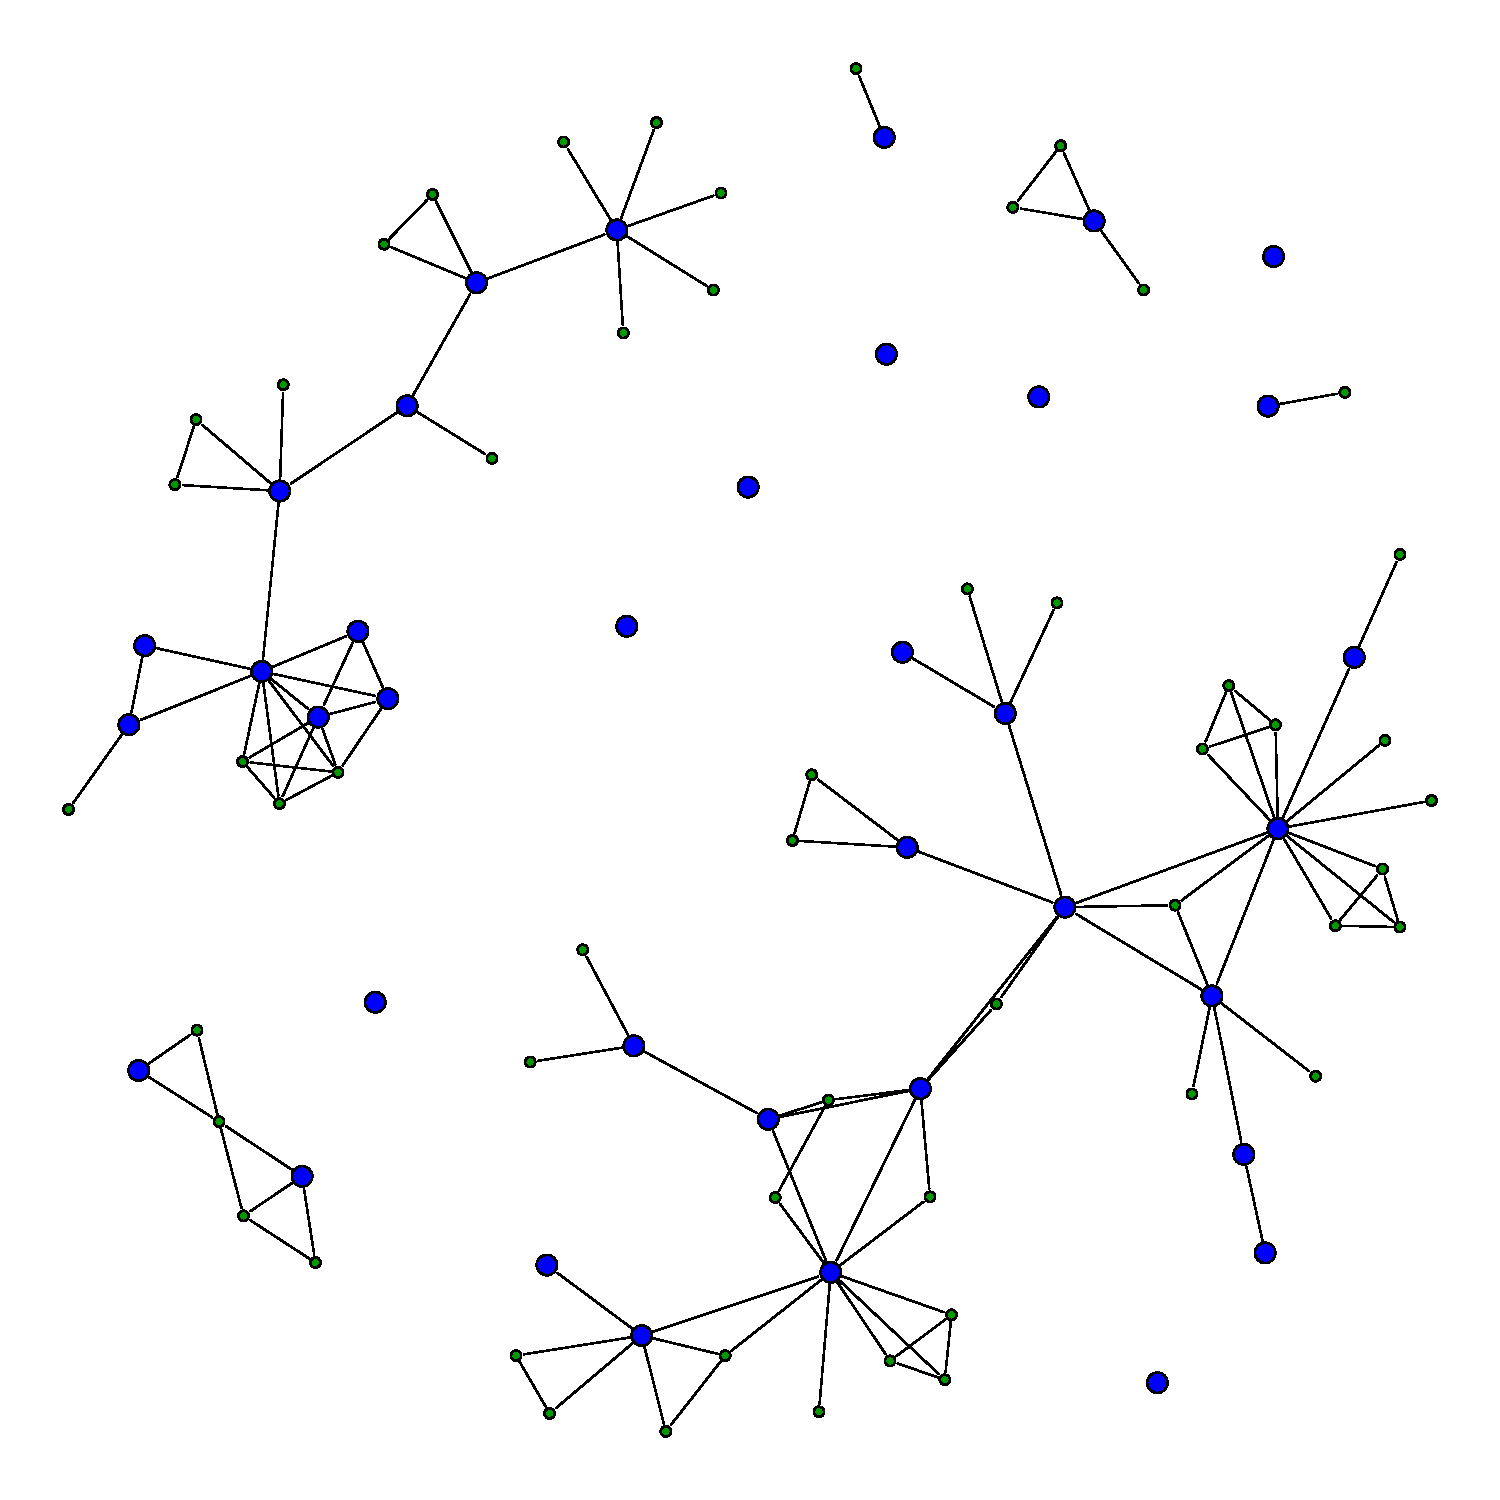
\includegraphics[width=.6\textwidth]{graph}
  \caption{Exemplo de grafo simples.}
  \label{fig:humanbeta}
\end{figure}

\begin{figure}
  \centering
  \begin{subfigure}{0.4\textwidth}
    \centering
    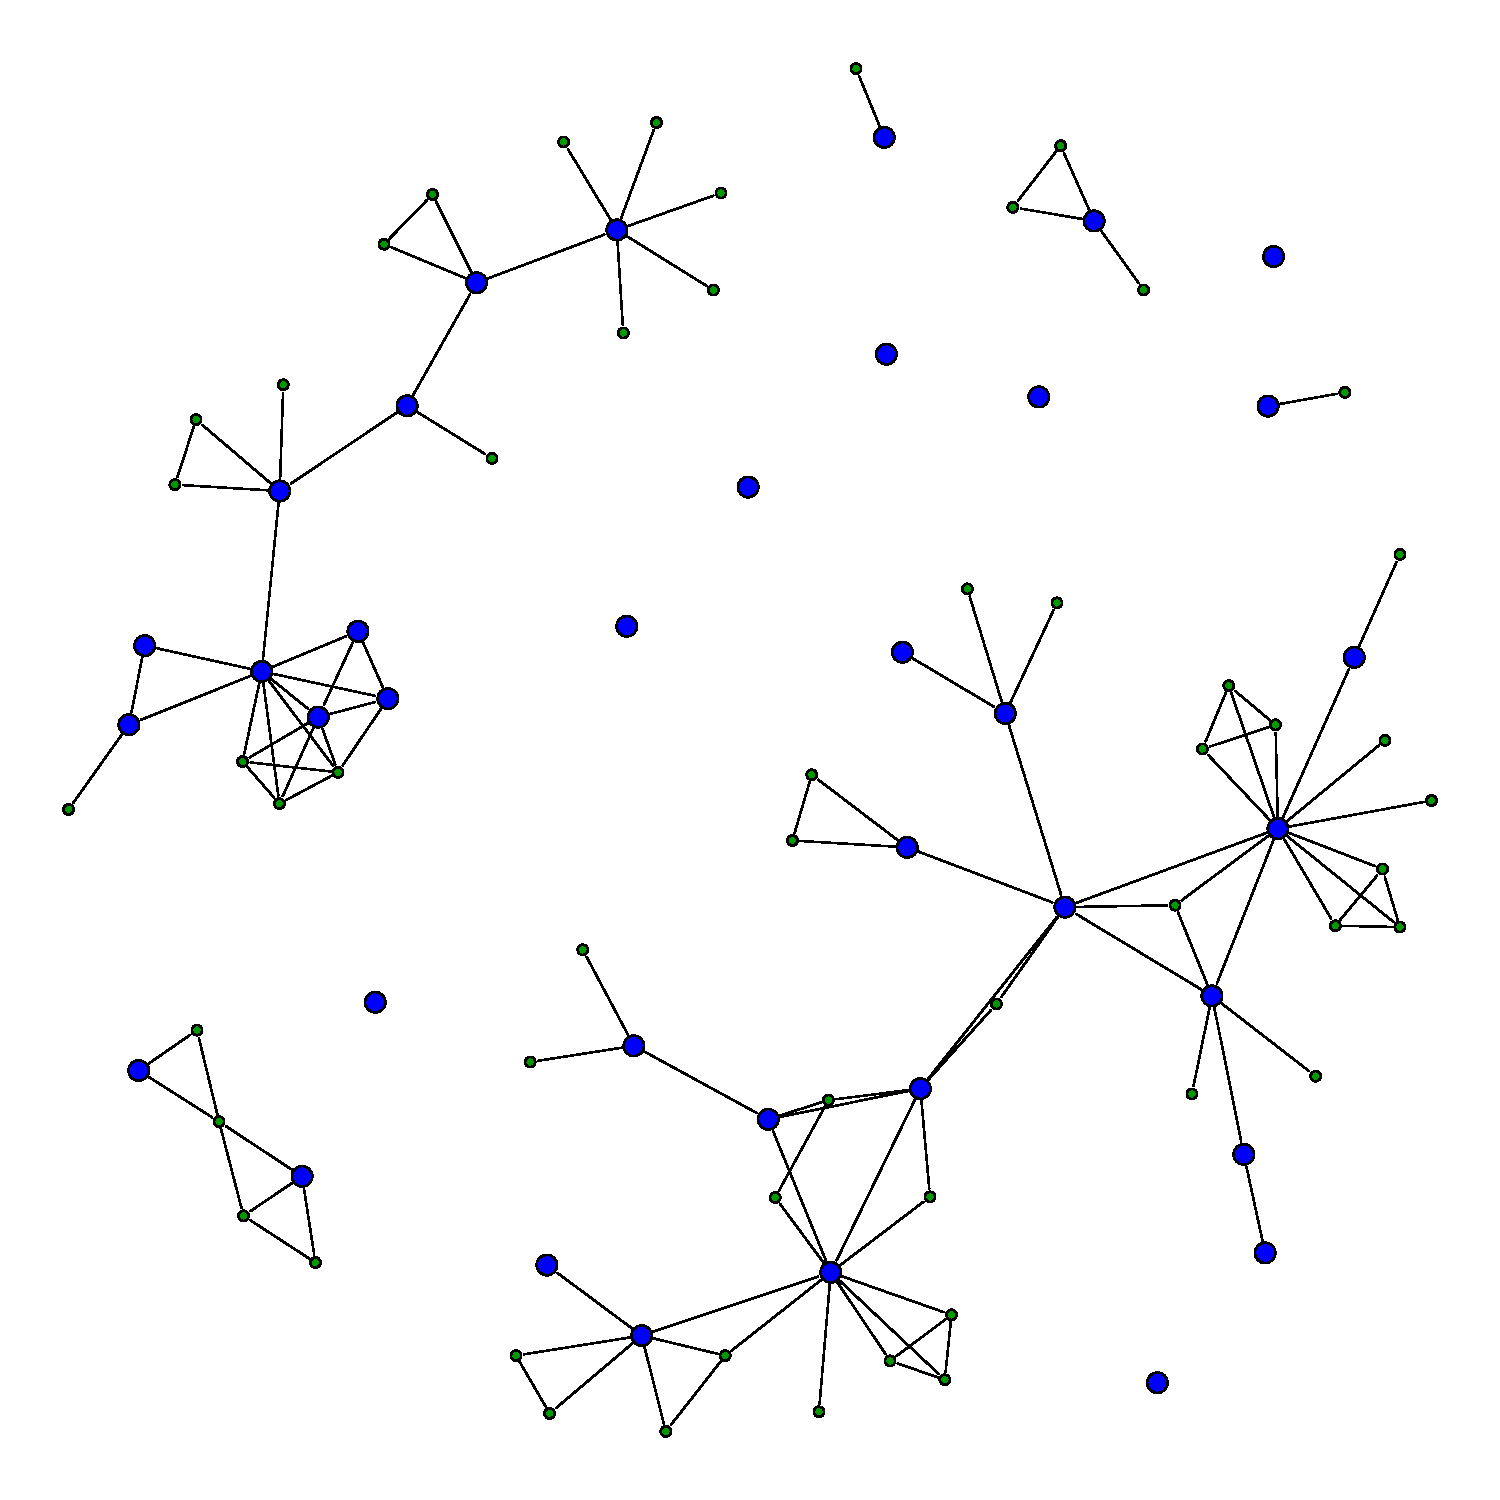
\includegraphics[width=.7\textwidth]{graph}
    \caption{O mesmo exemplo.}
    \label{fig:subfigures:a}
  \end{subfigure}
  \begin{subfigure}{0.4\textwidth}
    \centering
    \begin{turn}{90}
      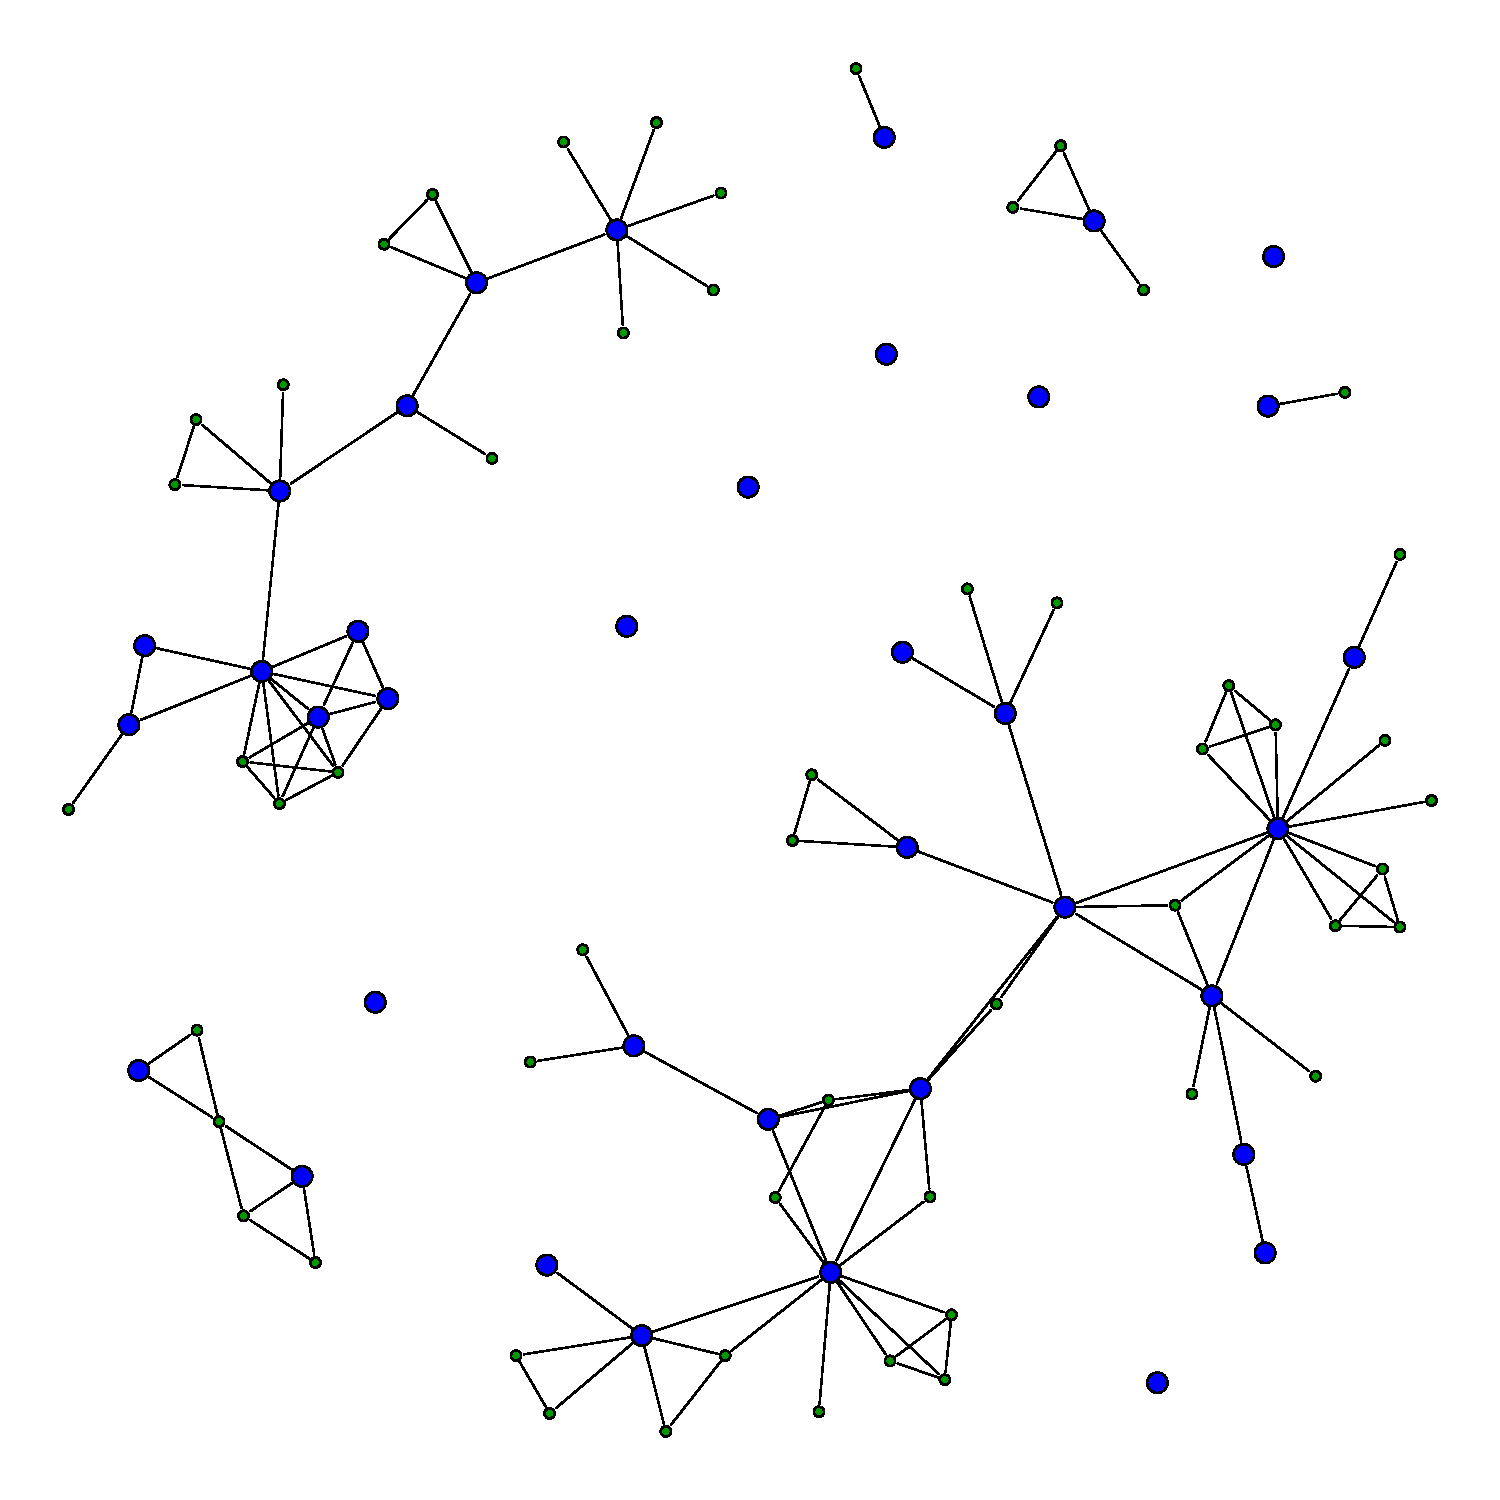
\includegraphics[width=.7\textwidth]{graph}
    \end{turn}
    \caption{O mesmo exemplo, girado.}
    \label{fig:subfigures:b}
  \end{subfigure}
  \caption{Exemplo de subfiguras.}
  \label{fig:subfigures}
\end{figure}


% Foi utilizado o pacote listings para formatar o código fonte
% Veja no preambulo do arquivo tese-exemplo.tex os parâmetros de configuração.
\begin{figure}
  \index{Java}
  \centering
\begin{lstlisting}[language=Java, style=wider]
for (i = 0; i < 20; i++)
{
	// Comentário
	System.out.println("Mensagem...");
}
\end{lstlisting}
  \caption{Exemplo de laço em Java.}
  \label{fig:java}
\end{figure}

Talvez você precise organizar a apresentação da informação na forma de
tabelas\index{Floats}. Há diversos estilos de tabela; um exemplo simples é a
Tabela~\ref{tab:amino_acidos}. A Tabela~\ref{tab:ficha} mostra como construir
uma tabela em forma de ficha larga que deve ser impressa em modo paisagem (ela
é um \textit{float}, mas sempre é impressa em uma página separada). Outro
exemplo de tabela em modo paisagem, esta distribuída em duas páginas (sem ser
um \textit{float}), está no Apêndice \ref{ape:sequencias}\footnote{
Observe que o nome do Apêndice (``\ref{ape:sequencias}'') foi impresso em uma
linha separada, o que não é muito bom visualmente. Para evitar que isso
aconteça (não só no final do parágrafo, mas em qualquer quebra de linha),
faça o que já foi discutido na Seção~\ref{orphanchar} sobre símbolos
matemáticos: utilize um espaço não-separável para fazer referências a
figuras, tabelas, seções etc.: ``\textsf{... está no
Apêndice\textasciitilde\textbackslash{}ref\{ape:sequencias\}}''.}.

\begin{table}
\centering
  \hspace*{\fill}
  \begin{subtable}[b]{0.42\textwidth}
    \centering
    \begin{tabular}{ccl}
      \toprule
      Código & Abreviatura & \makecell{Nome\\completo} \\
      \midrule
      \texttt{A}      & Ala                   & Alanina \\
      \texttt{C}      & Cys                   & Cisteína \\
      ...             & ...                   & ... \\
      \texttt{W}      & Trp                   & Triptofano \\
      \texttt{Y}      & Tyr                   & Tirosina \\
      \bottomrule
    \end{tabular}
    \caption{Uma tabela simples.}
  \end{subtable}
  \hspace*{\fill}\hspace*{\fill}\hspace*{\fill}
  \begin{subtable}[b]{0.37\textwidth}
    \centering
    \begin{tabular}{ccl}
      \rothead{Código} & \rothead{Abreviatura} & \rothead{Nome\\completo} \\
      \midrule
      \texttt{A}      & Ala                   & Alanina \\
      \texttt{C}      & Cys                   & Cisteína \\
      ...             & ...                   & ... \\
      \texttt{W}      & Trp                   & Triptofano \\
      \texttt{Y}      & Tyr                   & Tirosina \\
      \bottomrule
    \end{tabular}
    \caption{Com cabeçalhos girados.}
  \end{subtable}
  \hspace*{\fill}
  \caption{Códigos, abreviaturas e nomes dos aminoácidos.}
  \label{tab:amino_acidos}
\end{table}

% Aumenta o espaçamento entre as linhas da tabela (default: 0pt)
\setlength\extrarowheight{4pt}

% sidewaystable e comandos relacionados são definidos na package rotating
\begin{sidewaystable}
\centering
\begin{tabular}{|M{0.265}|M{0.073}|M{0.084}|M{0.073}|M{0.073}|M{0.08}|M{0.082}|M{0.067}|}
  \hline
    \textbf{Experimento número:} & \multicolumn{2}{c|}{1} & \multicolumn{4}{c|}{\textbf{Data:}} & jan 2017
  \tabularnewline \hline
    \textbf{Título:} & \multicolumn{7}{c|}{Medições iniciais}
  \tabularnewline \hline
    \textbf{Tipo de experimento:} & \multicolumn{7}{c|}{Levantamento quantitativo}
  \tabularnewline \hline \hline
    \textbf{Locais}          & São Paulo & Rio de Janeiro & Porto Alegre & Recife & Manaus & Brasília & Rio Branco
  \tabularnewline \thickhline
    \textbf{Valores obtidos} & 0.2       & 0.3            & 0.2          & 0.7    & 0.5    & 0.1      & 0.4
  \tabularnewline \hline
\end{tabular}
\caption{Exemplo de tabela similar a uma ficha.}
\label{tab:ficha}
\end{sidewaystable}

% Redefinindo para o valor default
\setlength\extrarowheight{0pt}

\par

%% ------------------------------------------------------------------------- %%
\chapter{Conclusões}
\label{cap:conclusoes}

Vale muito a pena a leitura do trabalho de
%Uri Alon \cite{alon09:how}, % usando o estilo alpha
Uri \citet{alon09:how}, % usando o estilo plainnat
no qual apresenta-se
uma reflexão sobre a utilização da Lei de Pareto para tentar definir/escolher
problemas para as diferentes fases da vida acadêmica.  A direção dos novos
passos para a continuidade da vida acadêmica deveriam ser discutidos com seu
orientador.

\par
